% !TEX root = Bachelorarbeit_Paul_Zilewitsch.tex
\section{Konzipierung}

\subsection{Grundidee Webservice }


\subsection{UML - Modellierung}
\noindent
Grundlage der Modellierung bildet die grafische Notation Unifed Modeling Language (UML) in der Version 2.3. UML hat sich in den letzten Jahren bei der Erstellung objektorientierter Modelle bewährt und ermöglicht somit einheitliche Diagrammdarstellungen und Begriffsabgrenzungen. Deshalb kann UML als Standrad für die Modellierung objektorientierter Software gesehen werden.\footnote{Vgl. \citeauthor{Schneider} (\citeyear{Schneider}), S. 233.}\footnote{Vgl. \citeauthor{Balzert} (\citeyear{Balzert}), S. V.} \newline
Grundsätzlich werden zwei Sichtweisen in der UML unterschieden. Die nachfolgenden Tabelle erläutert die wichtigsten Unterschiede:

\begin{table}[h!]
    \begin{tabular}{ | p{2.5cm}| p{6cm} | p{6cm} |}
    \hline
    Diagrammtyp & Verhaltensdiagramm & Strukturdiagramm \\ \hline
   Sichtweise & dynamisch & statisch \\ \hline
   Beispiele & Aktivitätsdiagramm, Zustandsdiagramm, Sequenzdiagramm &  Klassendiagramm, 
   Objektdiagramm, Paketdiagramm\\ \hline
   Beschreibung &  Es werden die Komponenten des Systems erläutert, die sich während der Laufzeit 
   verändern. Dabei werden die Abläufe des Systems ersichtlich und auch inwiefern der Benutzer diese 
   beeinflusst & Aus dieser Sicht werden die Komponenten des Systems betrachtet, die unabhängig von 
   der Laufzeit sind. Ihre Ein-und Ausgabedaten können sich verändern, aber die Beziehungen zwischen 
   den Komponenten bleiben bestehen. \\ \hline  
    \end{tabular}
    \caption{UML-Diagrammtypen, Quelle: in Anlehnung an Schneider (2012) , S. 234.}
\end{table}


\noindent
Insgesamt gibt es sieben Verhaltens -und Strukturdiagramme. Es können nicht alle vierzehn Diagramme in dieser Arbeit platz finden und bei diesem Vorgehen würde auch der Fokus auf die wichtigsten Fragestellungen verloren  gehen. Aus diesem Grund wurden zwei Verhaltensdiagramme und ein Strukturdiagramm ausgewählt, die die Abläufe bei der Erweiterung des Service Desk von GEBman 10 ersichtlich machen und die Implementierung erleichtern sollen. \\

\noindent
Das erste Verhaltensdiagramm soll die Frage klären, welche Aktionen der Benutzer mit dem Versenden einer E-Mail ausführen kann und wie das System darauf reagiert. Im Punkt 4.2 wurde auf die Anforderungen der Erweiterung eingegangen. Diese werden nun mit dem Aktivitätsdiagramm  in der Abbildung~\ref{fig:Aktivitaetsdiagramm} erläutert.

\begin{figure}[h!]
\centering
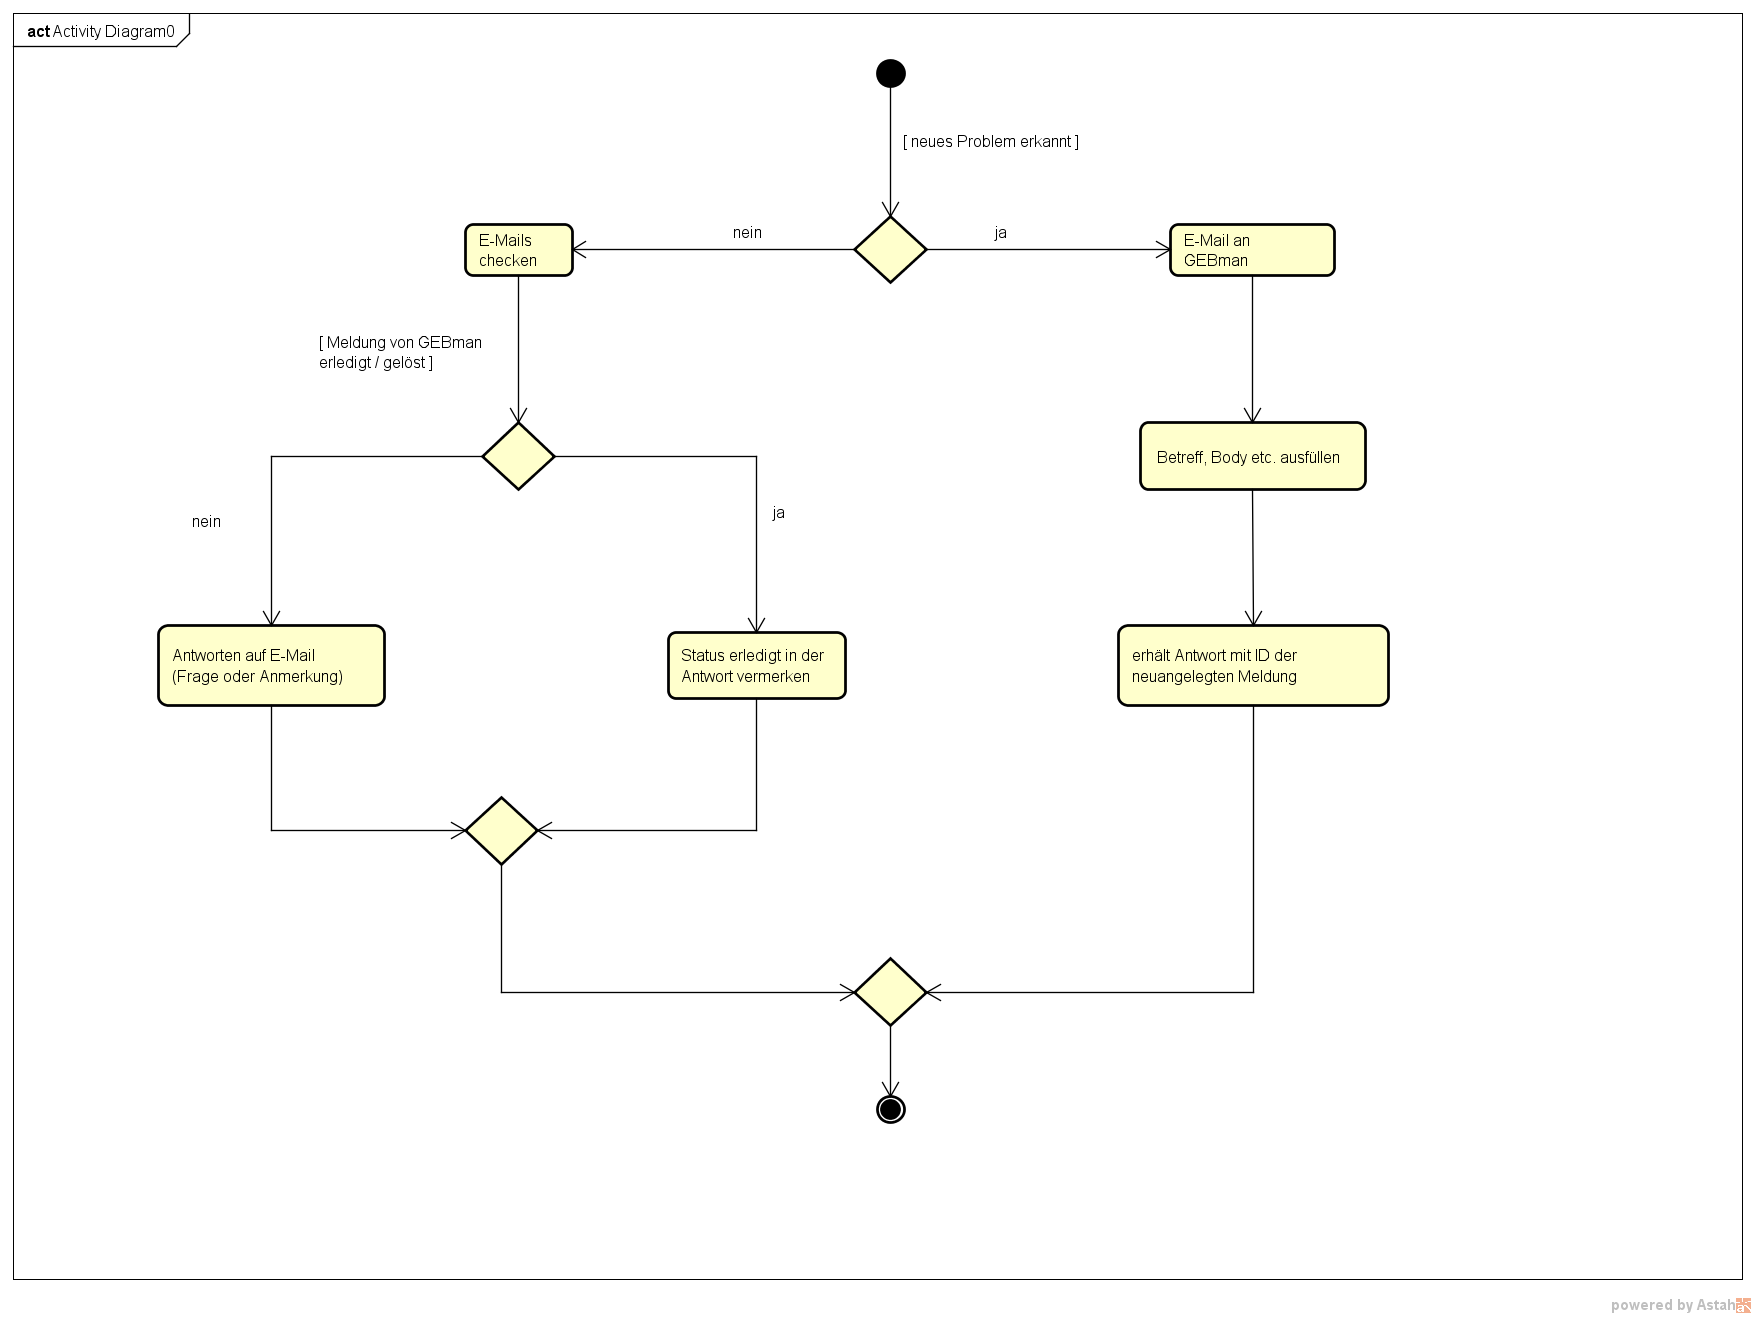
\includegraphics[width=0.65\textwidth]{Abbildungen/Aktivitaetsdiagramm.png}
	\caption[Aktivit{\"a}tsdiagramm]{Aktivit{\"a}tsdiagramm, Quelle: eigene Darstellung}
	\label{fig:Aktivitaetsdiagramm}
\end{figure}

\noindent
Die erste Fallentscheidung (F1), muss direkt zu Beginn vom Benutzer getroffen werden. \newline
Sollte er ein neues Problem erkannt haben, schickt er eine Mail an GEBman 10. Hierfür müssen die entsprechenden Parameter ausgefüllt werden. Wichtig ist, dass im Betreff der Vermerk \enquote{\#neu} eingetragen wird. GEBman 10 wertet diese Mail aus und legt eine neue Meldung im Service Desk an. Diese Meldung erhält eine eindeutige ID. Der Benutzer erhält anschließend eine Bestätigungsmail mit der ID der Meldung, wenn die Erstellung erfolgreich war.\newline
Möchte der Benutzer allerdings nur auf bereits bestehende Meldungen antworten, muss in anderer Weise vorgegangen werden. Entscheidet sich der Benutzer in der zweiten Fallentscheidung (F2), einer Meldung eine Antwort oder einen Anhang hinzuzufügen, so muss er die entsprechende ID der Meldung in den Betreff eintragen und kann dann die Antwort in den Mail Body eingeben. GEBman fügt dann die Antwort an die entsprechende Meldung mit der ID an oder fügt ihr einen Anhang hinzu.\newline
Natürlich kann er auch direkt auf eine Mail antworten, die er von GEBman erhalten hat, hierbei übernimmt das Mail-System automatisch den Betreff mit der entsprechenden ID. Der Benutzer hat außerdem die Möglichkeit, eine Meldung den Status \enquote{Fertig} zuzuweisen. Dafür muss in den Betreff der E-Mail der Vermerk \enquote{\#fertig}. Im Service Desk wird daraufhin die Meldung ebenfalls den Status \enquote{Fertig} annehmen.\\

\noindent
Anders als beim Aktivitätsdiagramm wird in der nachfolgenden Abbildung ein Zustandsdiagramm dargestellt. Die beiden Diagramme ähneln sich von ihrer Notation sehr, das Zustandsdiagramm legt aber mehr Fokus auf die Zustände des Systems, die es während der Laufzeit annehmen kann. Deshalb ist es auch das zweite Verhaltensdiagramm. Hierbei ist es wichtig, dass immer ein Ereignis eintreffen muss, damit das System in ein anderen Zustand wechseln kann.\footnote{Vgl. \citeauthor{Balzert} (\citeyear{Balzert}), S. 40.}

\begin{figure}[h!]
\centering
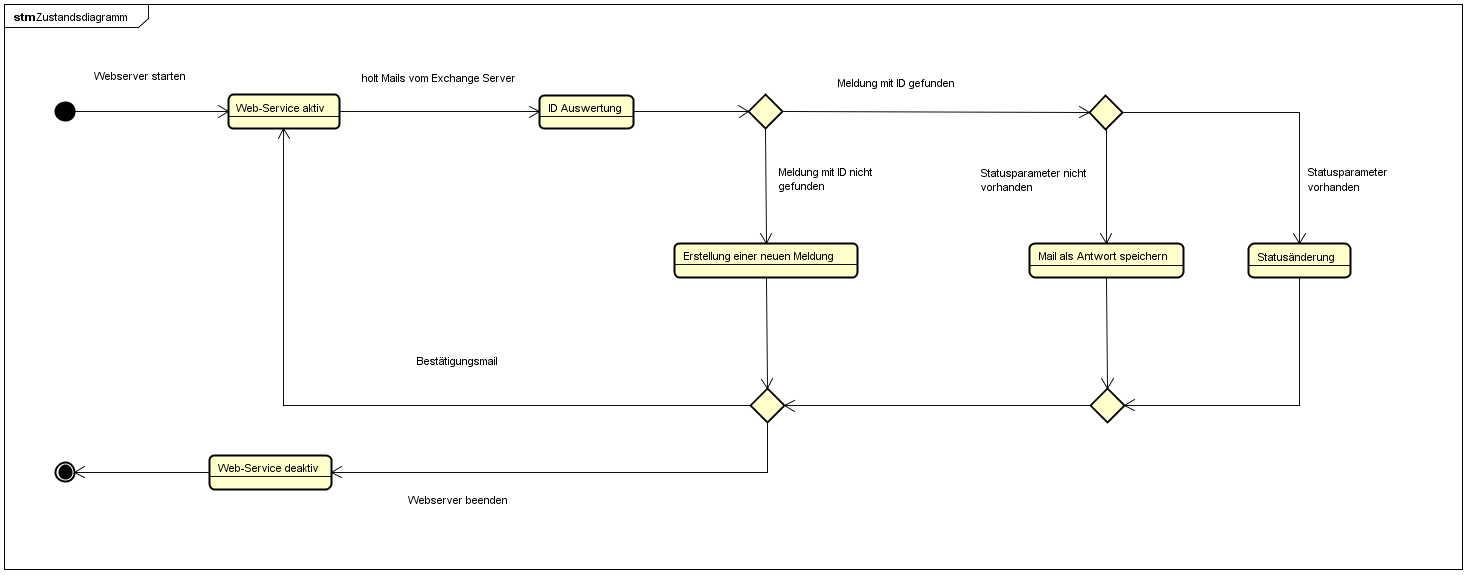
\includegraphics[width=0.95\textwidth]{Abbildungen/Zustandsdiagramm.png}
	\caption[Zustandsdiagramm]{Zustandsdiagramm, Quelle: eigene Darstellung}
	\label{fig:Zustandsdiagramm}
\end{figure}

\noindent
Sobald der Webserver gestartet ist, ist Anfangszustand der aktive Web-Service in GEBman 10 . In regelmäßigen Zeitabständen, werden über den WebService die neuesten Mails von dem Exchange Server geholt. Dann werden die in der Betreffzeile der Mail befindlichen ID's ausgewertet. Ist keine ID vorhanden, aber der Vermerk \enquote{\#neu} enthalten, geht der Web-Service in den Zustand einer neuen Meldungserstellung über. Anschließend wird die Bestätigungsmail versendet\newline
Ist in der Meldung allerdings eine ID vorhanden, wird zunächst einen Status-Vermerk geprüft. Sollte keiner enthalten sein, tritt der Zustand ein, in dem der Mail-Body als Antwort der Meldung hinzugefügt wird. Ist ein jedoch ein Status-Vermerk vorhanden, ändert der Web-Service den Status der zugehörigen Meldung.\newline
Nachdem das Intervall abgeschlossen ist, wechselt der Web-Service in den aktiven/wartenden Zustand und holt sich im nächsten Intervall die Mails vom Exchange Server. Nur wenn der Webserver beendet wird, ist logischerweise auch der Web-Service deaktiviert. Ansonsten soll er permanent laufen.\\

\noindent
Die Verhaltensdiagramme aus Benutzer -und Systemperspektive sind somit abgeschlossen. Das Klassendiagramm in Abbildung ~\ref{fig:Klassendiagramm} ist ein Strukturdiagramm, dass einen groben Überblick in den zu implementierenden Web-Service und der Beziehung zu dem restlichen System geben soll.




\begin{figure}[h!]
\centering
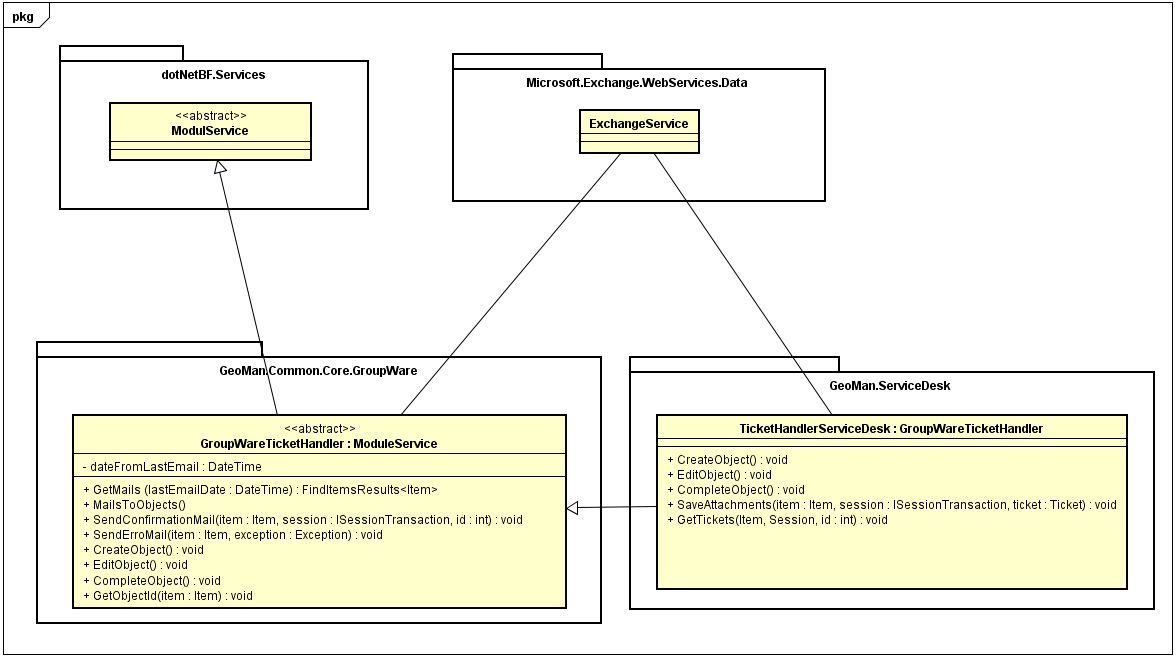
\includegraphics[width=0.75\textwidth]{Abbildungen/Klassendiagramm.png}
	\caption[Klassendiagramm]{Klassendiagramm, Quelle: eigene Darstellung}
	\label{fig:Klassendiagramm}
\end{figure}




\subsection{Zielsetzung}
\subsection{Sicherheitsaspekte}
\noindent
Immer wieder vernachlässigen Entwickler die Sicherheit ihrer Implementierungen. Das liegt meistens an mangelnder Zeit, da Releases einen festen Zeitplan verfolgen, den es einzuhalten gilt. Es kann aber auch sein, dass die Implementierung nicht aus dem Blickwinkel der Sicherheit betrachtet wird. "Hauptsache es funktioniert erst einmal", wird dann häufig als Argument genutzt. Natürlich hat das wenig mit Sicherheit zu tun. Dabei können es Entwickler mit wenig Aufwand, Angreifern deutlich schwerer machen. Deswegen werden im nachfolgendem zwei Sicherheitsprobleme für die Umsetzung des Konzepts in GEBman 10 besprochen. Die Abbildung XX zeigt zwei kritische Bereiche, die genauer erläutert werden müssen.

\begin{figure}[h!]
\centering
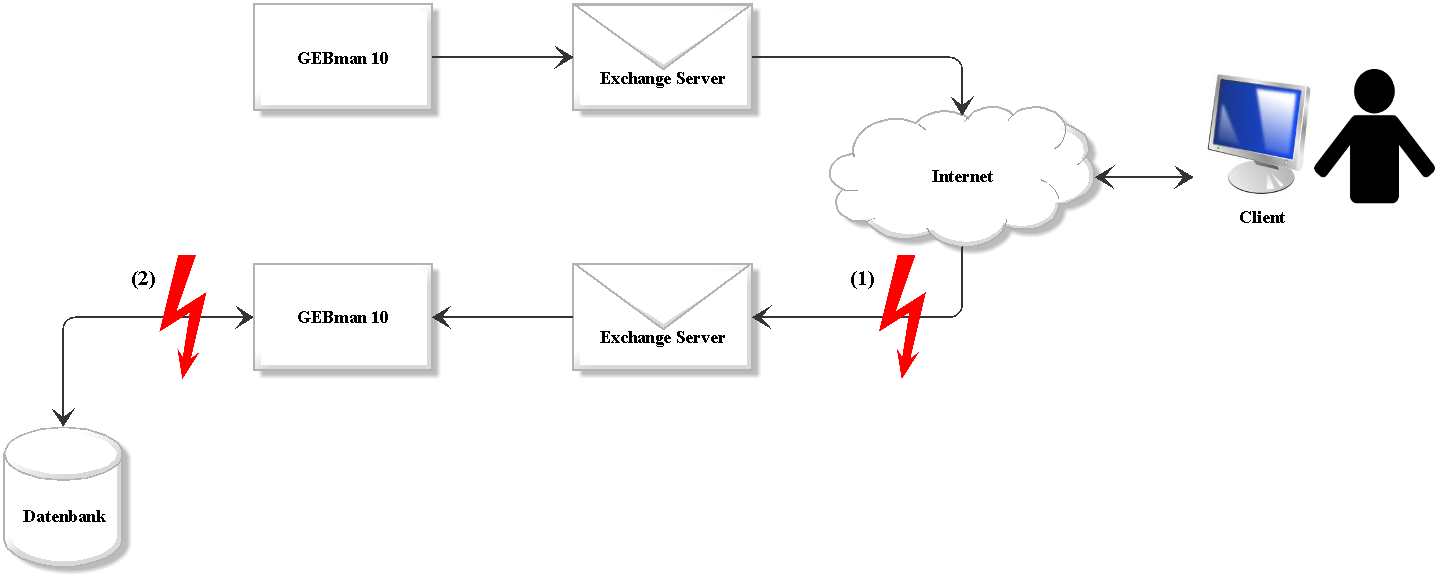
\includegraphics[width=0.85\textwidth]{Abbildungen/Sicherheitsprobleme.png}
	\caption[Sicherheitsprobleme]{Sicherheitsprobleme, Quelle: eigene Darstellung}
	\label{fig:Sicherheitsprobleme}
\end{figure}

\noindent
Der rechte rote Blitz - gekennzeichnet mit der (1) - symbolisiert das erste Problem.

\noindent
Beim zweiten roten Blitz der Abbildung XX - gekennzeichnet mit der (2) - wird uns die Arbeit nicht wie beim ersten kritischen Bereich abgenommen. GEBman 10 synchronisiert in regelmäßigen Abständen die Nachrichten vom hinterlegten Exchange Server. Entsprechend ihrer ID werden die Nachrichten in die Datenbank von GEBman 10 gespeichert. Nun könnte ein Angreifer beispielsweise versuchen, in den Mail-Body versteckte SQL -Anweisungen oder JavaScript-Code einzuschleusen. Werden die SQL-Anweisungen in die Datenbank geschrieben, ohne sie vorher zu validieren, könnte der Angreifer Informationen über Daten in der Datenbank erlangen. Im schlimmsten Fall könnte er sie zerstören. Diese Angriffstmethode nennt sich SQL-Injection und zielt darauf ab, die normalen SQL-Statements mittels Sonderzeichen zu manipulieren. Selbst einfache Zeichen wie "--" können bewirken, dass alles, was hinter den beiden Bindestrichen steht, ignoriert wird. In T-SQL sind die beiden Bindestriche das Zeichen für einen Kommentar.
\noindent
Bei JavaScript-Code haben wir ein ähnliches Problem mit bestimmten Zeichen. Wird zum Beispiel die einfache Zeichenfolge "<script>alert('hallo')<script>" in die Datenbank geschrieben, passiert ersst einmal gar nichts. Die SQL-Statements werden hierdruch nicht manipuliert. Doch wird diese Zeichenfolge beispielsweise als Antwort auf eine Meldung geladen, erkennt der Browser möglicherweise JavaScript-Code anstatt einfachen Text. Das hat in unserem Beispiel zur Folge, dass der Browser eine kleine Nachricht meldet (siehe Abbildung).
Auch hier muss vor dem Einfügen der Zeichenfolge, eine Validierung vollzogen werden. Welche Zeichen genau gefiltert werden müssen, wird im Punkt 5 Umsetzung erläutert. Man sollte sich jedoch nicht darauf verlassen, dass die Schutzmechanismen des Microsoft Exchange Servers alle Zeichen und Zeichenfolgen als Bedrohung erkennen. Zeichen wie "--" oder ">" können durchaus im normalen Schriftverkehr gebräuchlich sein.
\noindent
Es gibt für Angreifer noch mehr Angriffsmöglichkeiten beispielsweise zwischen Client und Internet/Server über Man-in-the-Middle etc.. Darauf soll aber in dieser Arbeit nicht weiter eingegangen werden, da das ein sehr umfangreiches Thema ist und eine eigenständige Bachelorarbeit bilden könnte. Eins sollte jedem klar sein: Hat ein Cracker genügend Zeit und Ressourcen, ist ein System, das über das Internet kommuniziert, äußert schwer vollkommen zu sichern. 
\noindent
Durch die Analyse aus Punkt 2 und Punkt 3 konnte ein genaues Ziel gesetzt werden. Die Funktionsweise der Exchange Web Services sind geklärt und auch Sicherheitsaspekte wurden berücksichtigt. Die Konzipierung ist somit abgeschlossen und er Implementierung steht nichts mehr im Wege.
